The result in Theorem~\ref{adderr} justifies the use of WMPADP algorithm to MDPs with large state space. We demonstrate the usefulness of WMPADP algorithm by applying it to solve the `mountain-car' problem with a continuous state space.
\subsection{The Mountain Car Experiment}
The problem is to make an under-powered car climb a one-dimensional hill (Fig.~\ref{mcar}), whose position $x$ lies in the interval $[-1.2,0.5]$. There are $3$ actions available to the car, i.e., $A=\{0,1,2\}$. Here $a=0$ and $a=2$ correspond to accelerating to the left and the right respectively. Further, $a=1$ corresponds to no acceleration. The velocity $y$ is limited to $[-0.07,0.07]$. The dynamics is given by
\begin{align}
y_{t+1}&=y_t+0.001 (a_t-1)-0.0025 cos(3x_t),\\
x_{t+1}&=x_t+y_t.
\end{align}
The state space is continuous with $S=[-1.2,0.5]\times[-0.07,0.07]$ and the state is given by $s=(x,y), x\in [-1.2,0.5], y \in [-0.07,0.07]$. The goal-state is reached once the car crosses the position $x\geq 0.5$. The reward in the goal-state is $100$ and the reward is $0$ in all the other states. The feature vector for state $s=(x,y)$ is given by
\begin{align}\label{basisdef}
\phi^s=(\big|\beta(\frac{x+1.2}{1.7}-x_i)\big|^\gamma+\big|\beta(\frac{y+0.07}{0.14}-y_j)\big|^\gamma,\nn\\ 1\leq i,j\leq k)
\end{align}
where $\beta>0$ is a scaling factor, $\gamma>1$ is the order and $(x_i,y_j), i=1,\ldots,k, j=1,\ldots,k$ are the $k \times k$ centers. We let,
\begin{align}\label{centers}
x_1&=-1.2<x_2<\ldots<x_k=0.5,\\\mb&\text{ with}\mb x_{n+1}-x_n=\frac{1.7}{k-1},\mb 1<n<k.\nn\\ 
y_1&=-0.07<y_2<\ldots<y_k=0.07,\nn\\ \mb &\text{with} \mb y_{n+1}-y_n=\frac{0.14}{k-1},\mb 1<n<k-1.\nn
\end{align}
\begin{comment}
\begin{figure}
\begin{tikzpicture}
\begin{axis}
\addplot[only marks, black] plot file{cen.txt};
\end{axis}
\end{tikzpicture}
\label{gridp}
\caption{Various centers for the basis functions.}
\end{figure}
\end{comment}
\FloatBarrier
\begin{figure}[H]
\begin{tikzpicture}
\begin{axis}
\addplot3 [surf] gnuplot [raw gnuplot] {
set dgrid3d 50,50 spline;
splot './mfiles/basisf.dat';       
};
\end{axis}
\end{tikzpicture}
\caption{Basis Function centered at $(0,0)$.}
\label{basisf}
\end{figure}
It is easy to check that the feature vectors as defined in \eqref{basisdef} have the property given in \eqref{orth}. Further, the feature vector/basis function as defined in \eqref{basisdef} is the $\minp$ equivalent of radial basis functions in the conventional algebra, i.e., the basis function centered at $c=(x,y)$ takes a value equal to the multiplicative identity (in $\minp$ algebra) i.e., $0$, at the state $c$, and the values for states away from the $c$ tend towards the additive identity in $\minp$ algebra, i.e., $+\infty$. Fig.~\ref{basisf} shows the basis function centered at $(0,0)$.\\
%The WMPADP algorithm (Algorithm~\ref{algo2}) made use of $Z$ as in Definition~\ref{constsamp} with the set of states $\Ls$ given by $\Ls=\{(x_i^s,x_j^s), i=1,\ldots,k_1,j=1,\ldots,k_2\}$.\\
%We note that, it is difficult to perform the minimization in line-$3$ of Algorithm~\ref{algo1} over all $s \in S$ and hence we discretize $S$ by means of $k_1 \times k_1$ grid points. These grid points were generated by choosing $x^g_i, i=1,\ldots,k_1$ and $ y^g_j, j=1,\ldots,k_1$, with $s^g_{ij}=(x^g_i,y^g_j)$. 
\begin{comment}
\begin{figure}
\label{mcar}
\input{MOUNTAINCAR.pstex_t}
\caption{Mountain Car}
\end{figure}
\end{comment}
\FloatBarrier
\begin{figure}[H]
\begin{center}
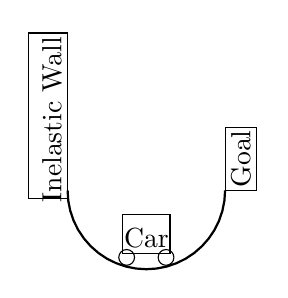
\begin{tikzpicture}
\draw [black,thick,domain=180:360] plot ({cos(\x)}, {sin(\x)});
\node [rotate=90] at (-1.2,0.9) { Inelastic Wall};
\draw (-1.5,-.1) rectangle (-1,2.0);
\node[] at (0,-0.6) { Car};
\draw (-0.3,-0.8) rectangle (0.3,-0.3);
\draw (1,0.0) rectangle (1.4,0.8);

\draw[] (-0.25,-0.85) circle(0.1);
\draw[] (0.25,-0.85) circle(0.1);
\node [rotate=90] at (1.2,0.4) { Goal};
\end{tikzpicture}
\end{center}
\caption{Mountain Car}
\label{mcar}
\end{figure}

In our experiments, we chose $\Ls=\{(x_i^s,y_j^s), 1\leq i,j \leq k_1\}$, where $x_i^s$ and $y_j^s$ were generated according to \eqref{centers} with $k=k_1$. We also fixed $\beta=100$ and $\gamma=2$, and varied $k=5, 7, 9, 11$ and $k_1=30,40,50$, the discount factor was set to $\alpha=0.95$, and $\epsilon=1e^{-5}$. The approximate value function computed by the WMPADP algorithm is shown in Fig.~\ref{ValFunc} and the actual value function is presented in Fig.~\ref{actvalfunc}. The approximate value functions computed in the various settings were used to generate corresponding greedy policies whose performance is shown in Table~\ref{episode}. The performance is evaluated via the number of steps taken by the car to reach the goal using the respective greedy policy.
\FloatBarrier
\begin{table}[H]
\begin{tabular}{|c|c|c|} \hline
$k$ & $k_1$ &Steps to reach the goal\\ \hline	
$5$ &30 &285 \\ \hline
5 &40 &285 \\ \hline
5 &50 &285 \\ \hline

7 &30 &322 \\ \hline
7 &40 &322 \\ \hline
7 &50 &327 \\ \hline

9 &30 &218 \\ \hline
9 &40 &317 \\ \hline
9 &50 &324 \\ \hline

11 &30 &267 \\ \hline
11 &40 &260 \\ \hline
11 &50 &257 \\ \hline
\end{tabular}
\caption{Number of steps taken by the $\emph{Greedy}$ policy}
\label{episode}
\end{table}
The near-optimal policy derived from the actual value function for this problem is known to achieve the goal within $150$ steps \cite{rl}. However, finding the actual value function in this case requires significantly more computation.
\FloatBarrier
\begin{figure}[H]
\begin{tikzpicture}
\begin{axis}
\addplot3 [surf] gnuplot [raw gnuplot] {
set dgrid3d 50,50 spline;
splot 'mfiles/val.dat';       
};
\end{axis}
\end{tikzpicture}
\caption{Actual Value Function Corresponding to the Mountain Car Problem}
\label{actvalfunc}
\end{figure}


\FloatBarrier
\begin{figure*}[H]
\begin{minipage}{1\textwidth}
\resizebox{\columnwidth}{!}{
\begin{tabular}{ccc}
   \begin{tikzpicture}
    \begin{axis}
    \addplot3 [surf] gnuplot [raw gnuplot] {
        set dgrid3d 30,30 spline;
        splot 'mfiles/data730.dat';       
    };
    \end{axis}
    \end{tikzpicture}
&
  \begin{tikzpicture}
    \begin{axis}
    \addplot3 [surf] gnuplot [raw gnuplot] {
        set dgrid3d 40,40 spline;
        splot 'mfiles/data740.dat';       
    };
    \end{axis}
    \end{tikzpicture}
&
  \begin{tikzpicture}
    \begin{axis}
    \addplot3 [surf] gnuplot [raw gnuplot] {
        set dgrid3d 50,50 spline;
        splot 'mfiles/data750.dat';       
    };
    \end{axis}
    \end{tikzpicture}\\
${k=5,k_1=30,V_{\max}=2.83e3 V_{\min}=0.73e3}$ & $k=5,k_1=40,V_{\max}=3.29e3, V_{\min}=0.74e3$	& $k=5,k_1=50,V_{\max}=3.20e3, V_{\min}=0.77e3$\\

   \begin{tikzpicture}
    \begin{axis}
    \addplot3 [surf] gnuplot [raw gnuplot] {
        set dgrid3d 30,30 spline;
        splot 'mfiles/data930.dat';       
    };
    \end{axis}
    \end{tikzpicture}
&
  \begin{tikzpicture}
    \begin{axis}
    \addplot3 [surf] gnuplot [raw gnuplot] {
        set dgrid3d 40,40 spline;
        splot 'mfiles/data940.dat';       
    };
    \end{axis}
    \end{tikzpicture}
&
  \begin{tikzpicture}
    \begin{axis}
    \addplot3 [surf] gnuplot [raw gnuplot] {
        set dgrid3d 50,50 spline;
        splot 'mfiles/data950.dat';       
    };
    \end{axis}
    \end{tikzpicture}\\
${k=7,k_1=30,V_{\max}=2.60e3, V_{\min}=0.45e3}$ &$k=7,k_1=40,V_{\max}=2.83e3, V_{\min}=0.47e3$	&$k=7,k_1=50,V_{\max}=2.80e3, V_{\min}=0.48e3$\\
   \begin{tikzpicture}
    \begin{axis}
    \addplot3 [surf] gnuplot [raw gnuplot] {
        set dgrid3d 30,30 spline;
        splot 'mfiles/data1130.dat';       
    };
    \end{axis}
    \end{tikzpicture}
&
  \begin{tikzpicture}
    \begin{axis}
    \addplot3 [surf] gnuplot [raw gnuplot] {
        set dgrid3d 40,40 spline;
        splot 'mfiles/data1140.dat';       
    };
    \end{axis}
    \end{tikzpicture}
&
  \begin{tikzpicture}
    \begin{axis}
    \addplot3 [surf] gnuplot [raw gnuplot] {
        set dgrid3d 50,50 spline;
        splot 'mfiles/data1150.dat'; 
    };
    \end{axis}
    \end{tikzpicture}\\
${k=11,k_1=30,V_{\max}=2.32e3, V_{\min}=0.18e3}$ &$k=11,k_1=40,V_{\max}=2.42e3, V_{\min}=0.20e3$	&$k=11,k_1=50,V_{\max}=2.42e3, V_{\min}=0.20e3$
\end{tabular}
}
\end{minipage}
\caption{Approximate Value Function for various values of $k$ and $k_1$}
\label{ValFunc}
\end{figure*}


